\section{Wizard Interface \& User Experience - Từ Code đến UI}

\subsection{Tổng quan về Wizard Interface}

Một trong những thay đổi quan trọng nhất từ notebook ban đầu là việc phát triển \textbf{Wizard Interface} - một giao diện người dùng thân thiện với 5 bước hướng dẫn chi tiết. Điều này chuyển đổi project từ một tool chỉ dành cho developers thành một platform accessible cho end users.

\subsection{Kiến trúc Wizard System}

\begin{minted}{bash}
wizard_ui/
├── __init__.py
├── core.py                 # Wizard management system
├── session_manager.py      # Session state management
├── validation.py           # Input validation system
├── navigation.py           # Navigation controller
├── components/             # Reusable UI components
│   ├── dataset_preview.py
│   └── file_upload.py
├── steps/                  # Individual wizard steps
│   └── step1_dataset.py
└── responsive/             # Responsive design components
\end{minted}

\subsection{5-Step Wizard Workflow}

Wizard Interface được thiết kế với 5 bước logic và tuần tự, mỗi bước có mục đích cụ thể và validation riêng:

\begin{enumerate}
    \item \textbf{Step 1: Dataset Selection \& Upload} - Chọn và tải dataset
    \item \textbf{Step 2: Column Selection \& Preprocessing} - Chọn cột và tiền xử lý dữ liệu  
    \item \textbf{Step 3: Model Configuration \& Vectorization} - Cấu hình mô hình và vectorization
    \item \textbf{Step 4: Training Execution \& Monitoring} - Thực thi training và theo dõi
    \item \textbf{Step 5: Results Analysis \& Export} - Phân tích kết quả và xuất dữ liệu
\end{enumerate}

\subsubsection{Bước 1: Lựa chọn và Tải lên Dataset}

\begin{figure}[H]
    \centering
    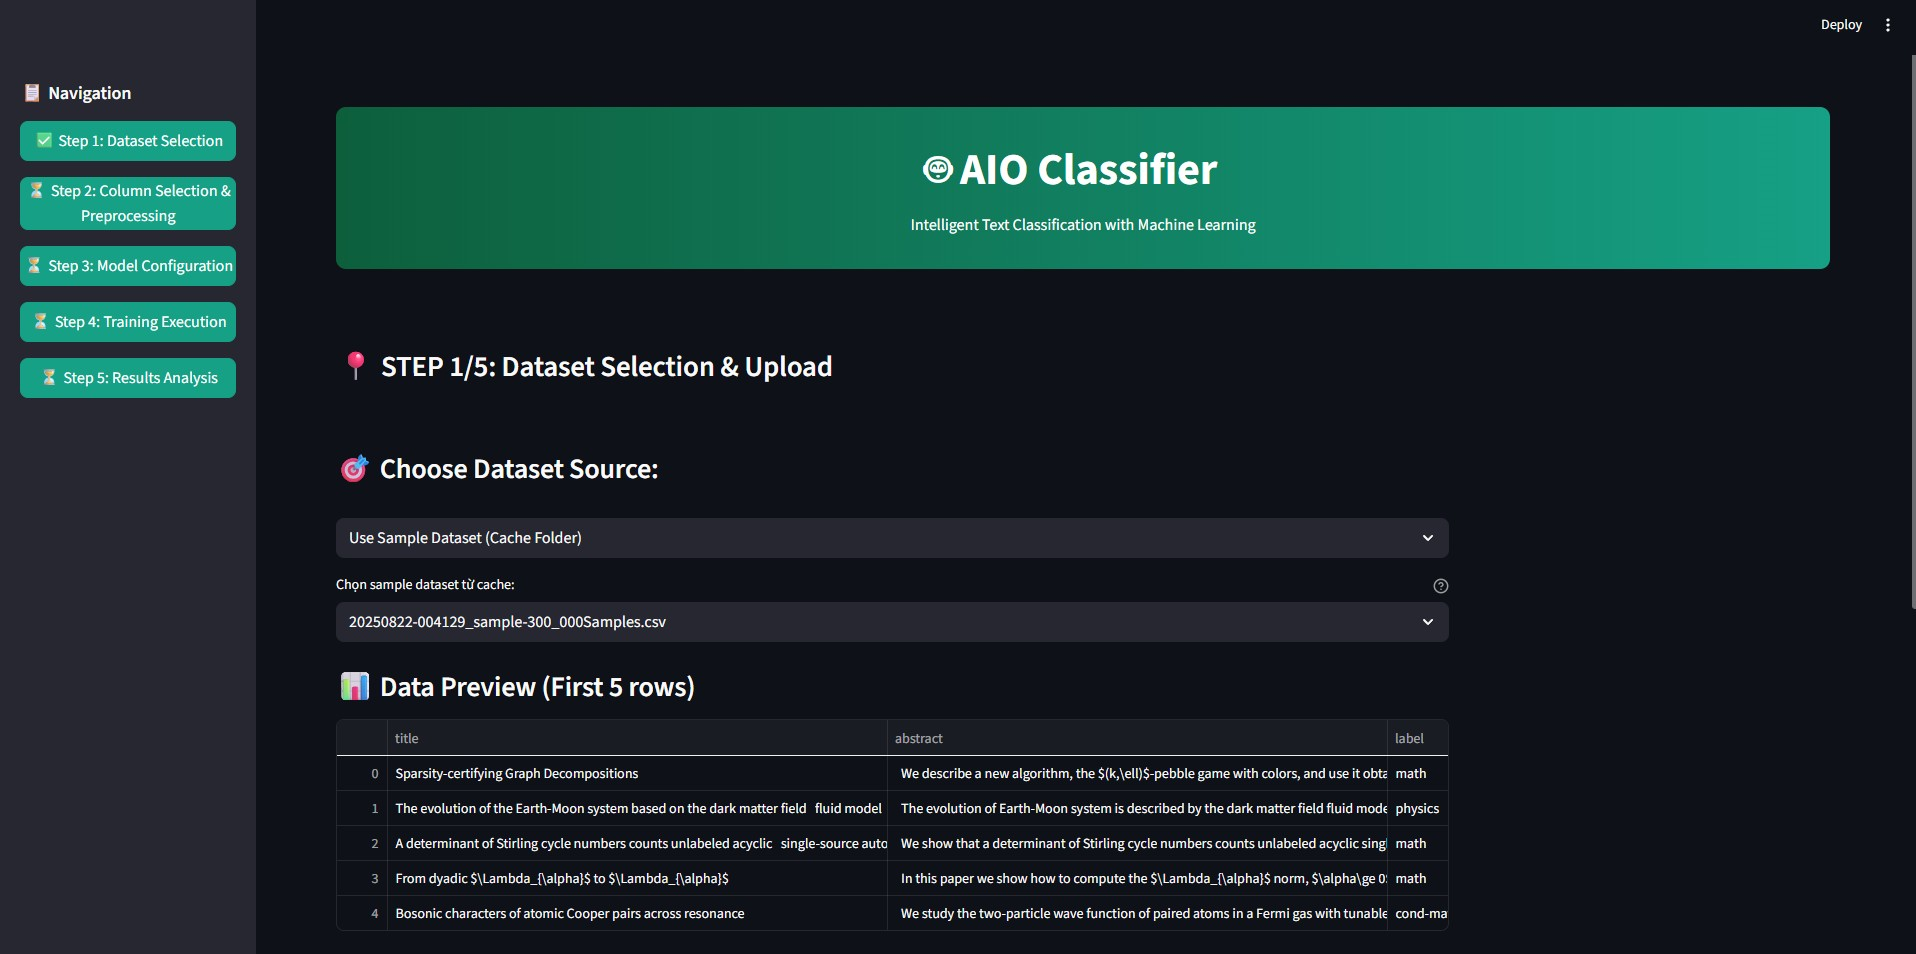
\includegraphics[width=0.9\textwidth]{image/Step 1.jpg}
    \caption{Bước 1: Giao diện Lựa chọn và Tải lên Dataset}
    \label{fig:step1}
\end{figure}

\textbf{Tính năng chính:}
\begin{itemize}
    \item \textbf{Lựa chọn nguồn Dataset:} Chọn giữa dataset ArXiv (khuyến nghị) hoặc tải lên dataset tùy chỉnh
    \item \textbf{Xem trước dữ liệu thời gian thực:} Hiển thị 5 dòng đầu tiên của dataset đã chọn với các cột title, abstract và label
    \item \textbf{Tùy chọn cấu hình:} Lựa chọn kích thước mẫu và hiển thị thống kê dataset
    \item \textbf{Xác thực đầu vào:} Thông báo lỗi và xác thực trước khi chuyển sang bước tiếp theo
    \item \textbf{Theo dõi tiến trình:} Các chỉ báo trực quan hiển thị trạng thái hoàn thành bước hiện tại
\end{itemize}

\textbf{Các thành phần giao diện:}
\begin{itemize}
    \item Panel điều hướng bên trái với các chỉ báo bước
    \item Dropdown nguồn dataset với tùy chọn ArXiv được chọn sẵn
    \item Bảng xem trước dữ liệu hiển thị các mục mẫu
    \item Nút Continue để chuyển sang bước tiếp theo
    \item Tooltip trợ giúp và các biểu tượng thông tin
\end{itemize}

\subsubsection{Bước 2: Lựa chọn Cột và Tiền xử lý}

\begin{figure}[H]
    \centering
    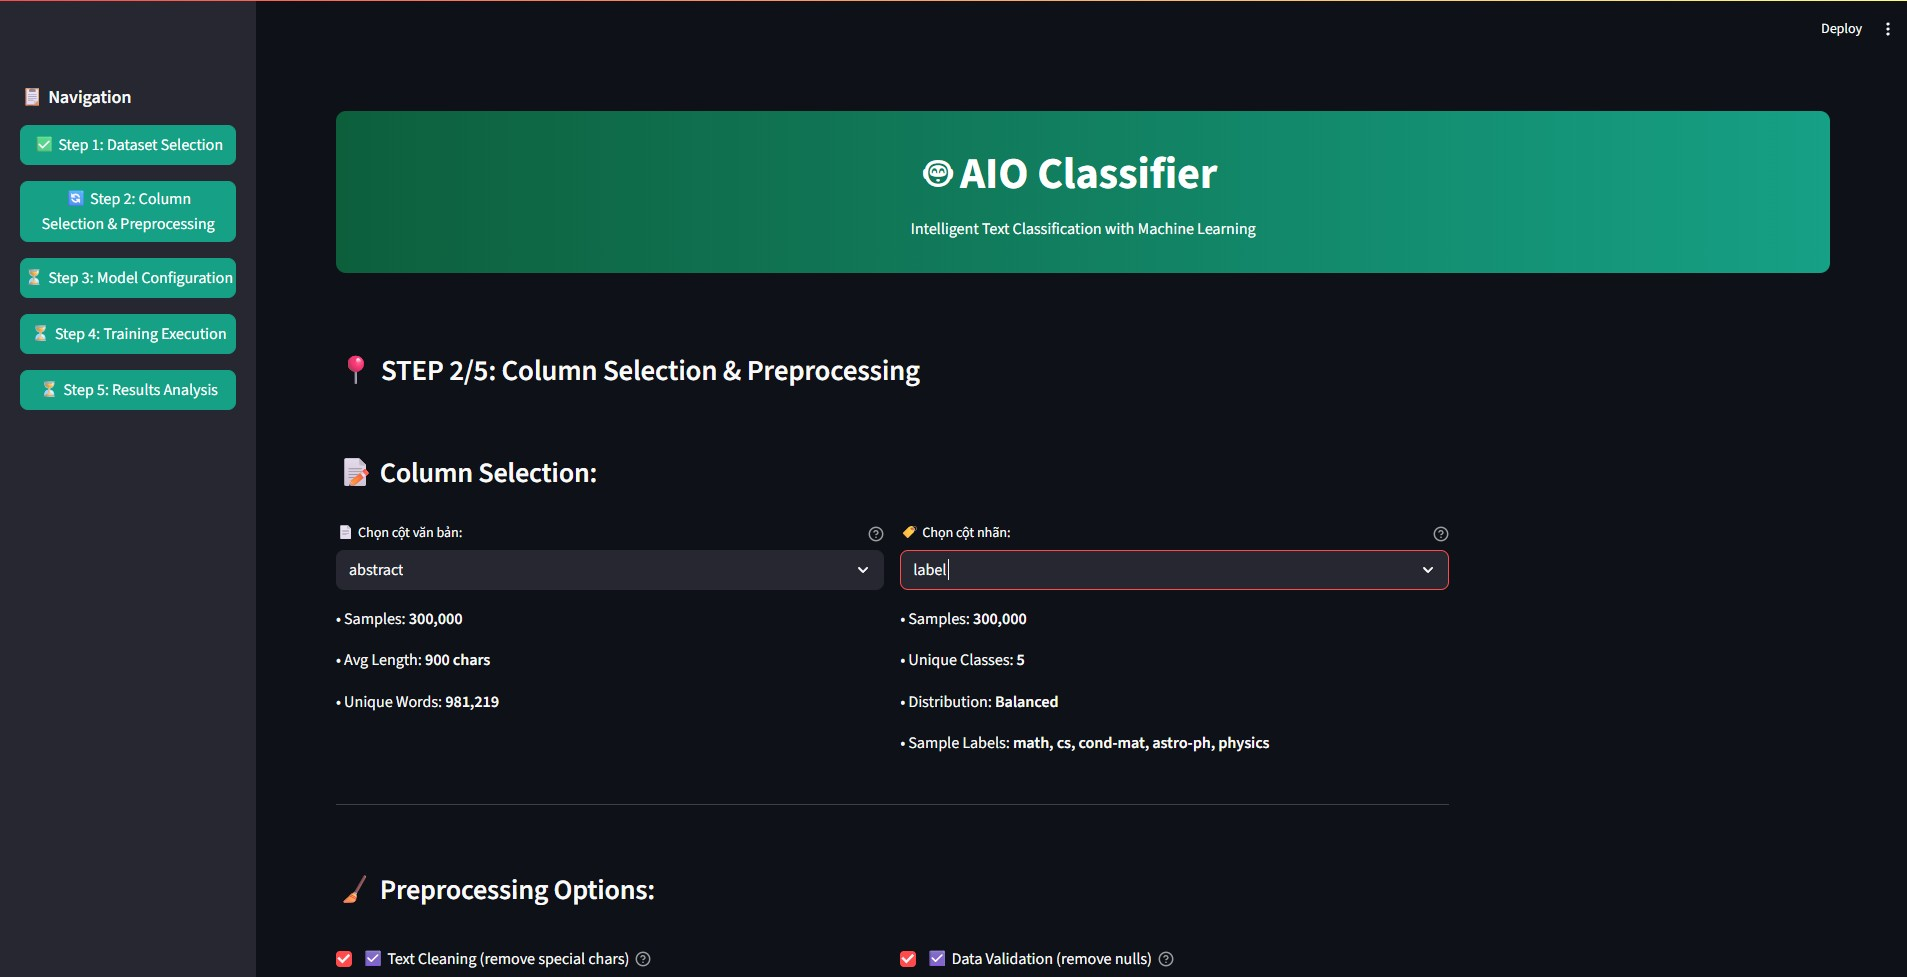
\includegraphics[width=0.9\textwidth]{image/Step 2.jpg}
    \caption{Bước 2: Giao diện Lựa chọn Cột và Tiền xử lý}
    \label{fig:step2}
\end{figure}

\textbf{Tính năng chính:}
\begin{itemize}
    \item \textbf{Lựa chọn cột:} Chọn cột văn bản (abstract) và cột nhãn (label) từ dataset
    \item \textbf{Thống kê thời gian thực:} Hiển thị số lượng mẫu, độ dài trung bình, từ duy nhất và phân phối lớp
    \item \textbf{Tùy chọn tiền xử lý:} Các checkbox làm sạch văn bản và xác thực dữ liệu
    \item \textbf{Theo dõi tiến trình:} Bước 1 hoàn thành (dấu tích xanh), Bước 2 đang hoạt động (được highlight)
    \item \textbf{Xác thực dữ liệu:} Xác thực tự động các cột đã chọn với thống kê
\end{itemize}

\textbf{Các thành phần giao diện:}
\begin{itemize}
    \item Dropdown cột văn bản được chọn sẵn là "abstract"
    \item Dropdown cột nhãn được chọn sẵn là "label"
    \item Hiển thị thống kê cho cả hai cột (300,000 mẫu, 5 lớp duy nhất)
    \item Các checkbox tiền xử lý cho làm sạch văn bản và xác thực dữ liệu
    \item Panel điều hướng hiển thị trạng thái hoàn thành các bước
\end{itemize}

\subsubsection{Bước 3: Cấu hình Mô hình và Vectorization}

\begin{figure}[H]
    \centering
    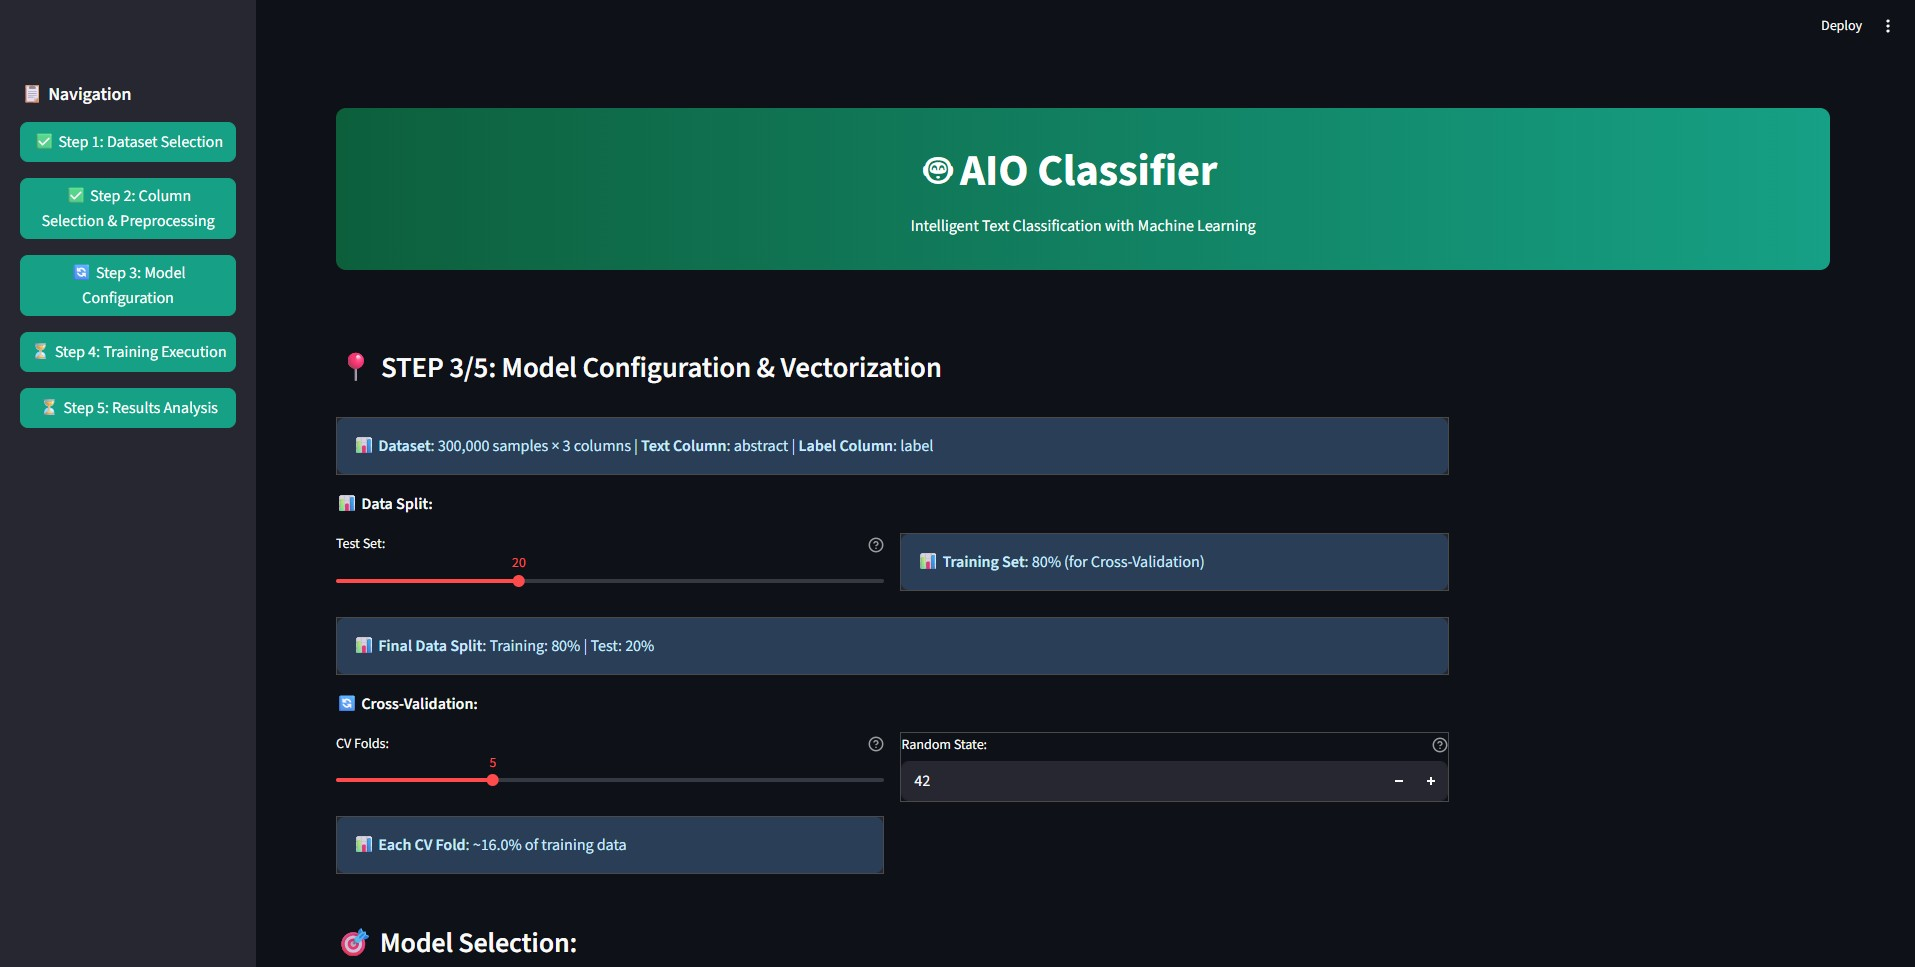
\includegraphics[width=0.9\textwidth]{image/Step 3.jpg}
    \caption{Bước 3: Giao diện Cấu hình Mô hình và Vectorization}
    \label{fig:step3}
\end{figure}

\textbf{Tính năng chính:}
\begin{itemize}
    \item \textbf{Cấu hình chia dữ liệu:} Thanh trượt test set (20\%) với tính toán training set (80\%)
    \item \textbf{Thiết lập Cross-Validation:} Thanh trượt CV folds (5 folds) với cấu hình random state
    \item \textbf{Hiển thị thông tin Dataset:} Hiển thị chi tiết dataset đã tải (300,000 mẫu × 3 cột)
    \item \textbf{Theo dõi tiến trình:} Bước 1-2 hoàn thành, Bước 3 đang hoạt động
    \item \textbf{Xem trước lựa chọn mô hình:} Chỉ ra các tùy chọn lựa chọn mô hình sắp tới
\end{itemize}

\textbf{Các thành phần giao diện:}
\begin{itemize}
    \item Thanh trượt phần trăm test set được đặt ở 20\%
    \item Thanh trượt Cross-validation folds được đặt ở 5
    \item Trường nhập Random state với giá trị 42
    \item Hộp tóm tắt dataset hiển thị thông tin cột
    \item Tính toán thời gian thực phần trăm training set và kích thước CV fold
    \item Panel điều hướng với các chỉ báo hoàn thành bước
\end{itemize}

\subsubsection{Bước 4: Thực thi Training và Giám sát}

\begin{figure}[H]
    \centering
    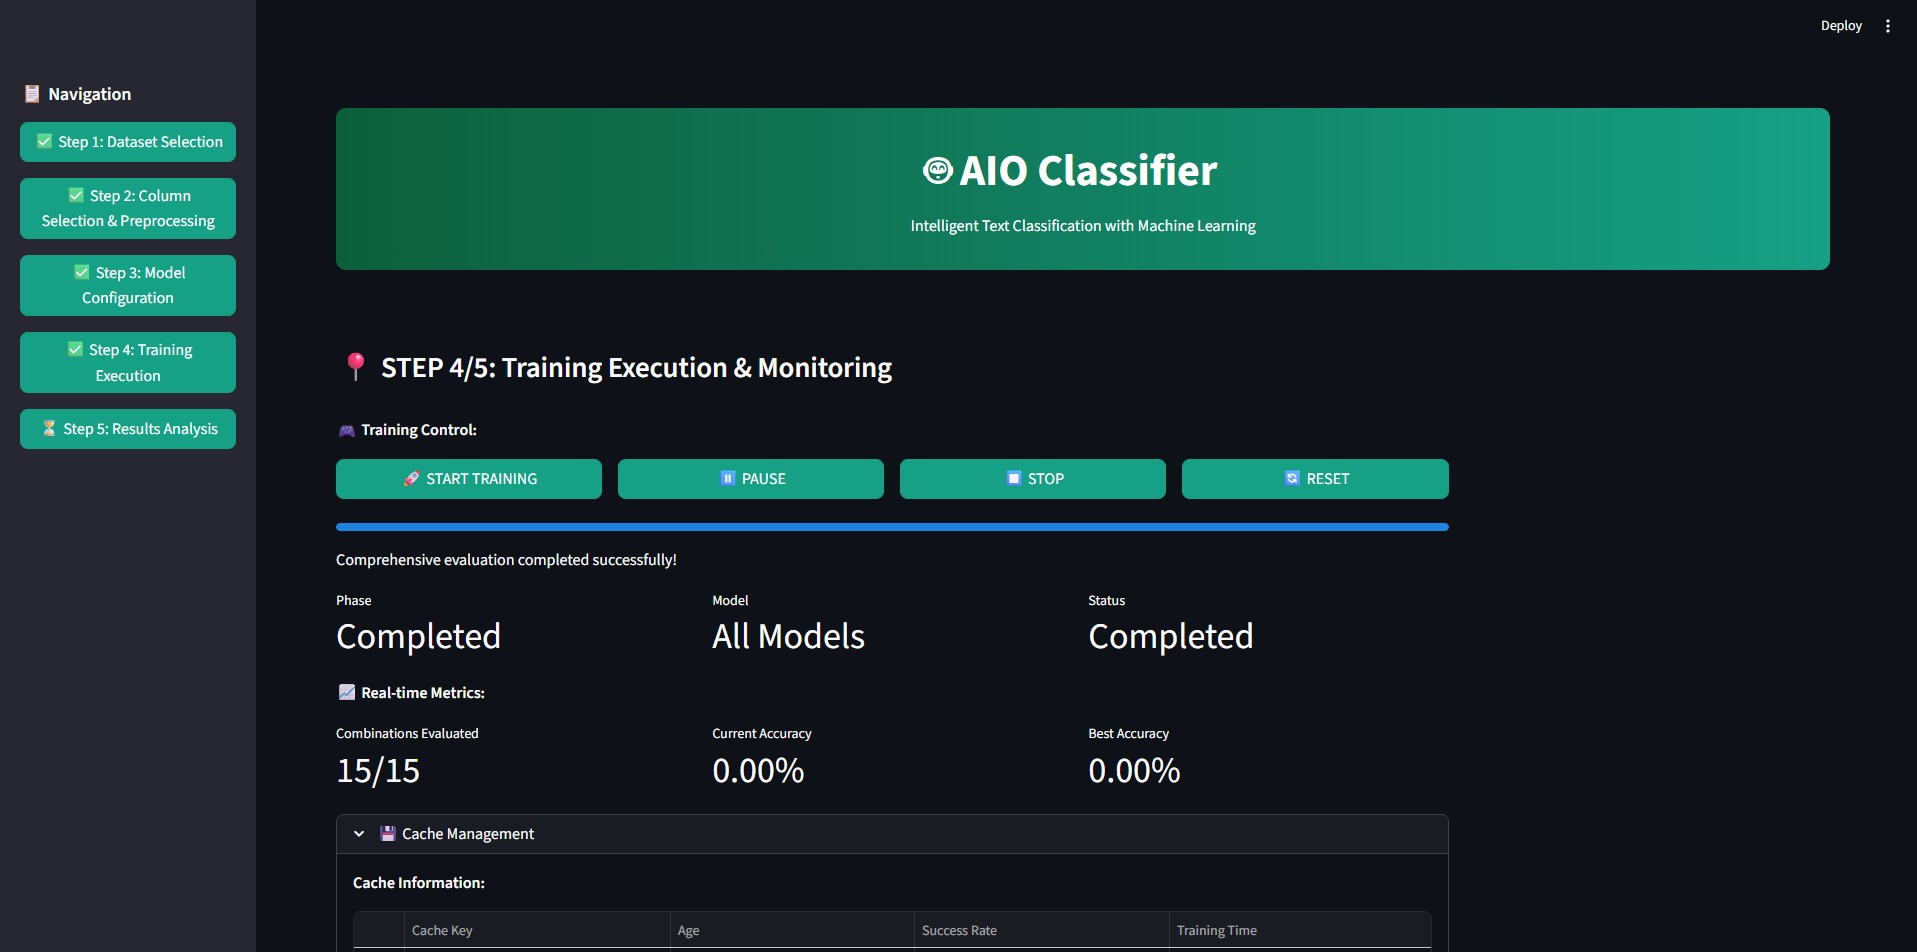
\includegraphics[width=0.9\textwidth]{image/Step 4.jpg}
    \caption{Bước 4: Giao diện Thực thi Training và Giám sát}
    \label{fig:step4}
\end{figure}

\textbf{Tính năng chính:}
\begin{itemize}
    \item \textbf{Bảng điều khiển Training:} Các nút START TRAINING, PAUSE, STOP và RESET
    \item \textbf{Cập nhật trạng thái thời gian thực:} Hiển thị "Comprehensive evaluation completed successfully!"
    \item \textbf{Theo dõi tiến trình:} Tất cả bước 1-4 hoàn thành với dấu tích xanh
    \item \textbf{Chỉ số hiệu suất:} Hiển thị số kết hợp đã đánh giá (15/15) và điểm accuracy
    \item \textbf{Quản lý Cache:} Phần có thể thu gọn cho thông tin cache và thống kê
\end{itemize}

\textbf{Các thành phần giao diện:}
\begin{itemize}
    \item Các nút điều khiển training với biểu tượng
    \item Thông báo trạng thái hiển thị trạng thái hoàn thành
    \item Tóm tắt training hiển thị "All Models" và trạng thái "Completed"
    \item Hiển thị chỉ số thời gian thực (0.00\% accuracy - cho thấy training đang tiến hành)
    \item Dropdown quản lý cache với bảng kết quả trống
    \item Panel điều hướng hiển thị tất cả các bước trước đã hoàn thành
\end{itemize}

\subsubsection{Bước 5: Phân tích Kết quả và Xuất dữ liệu - Tổng quan}

\begin{figure}[H]
    \centering
    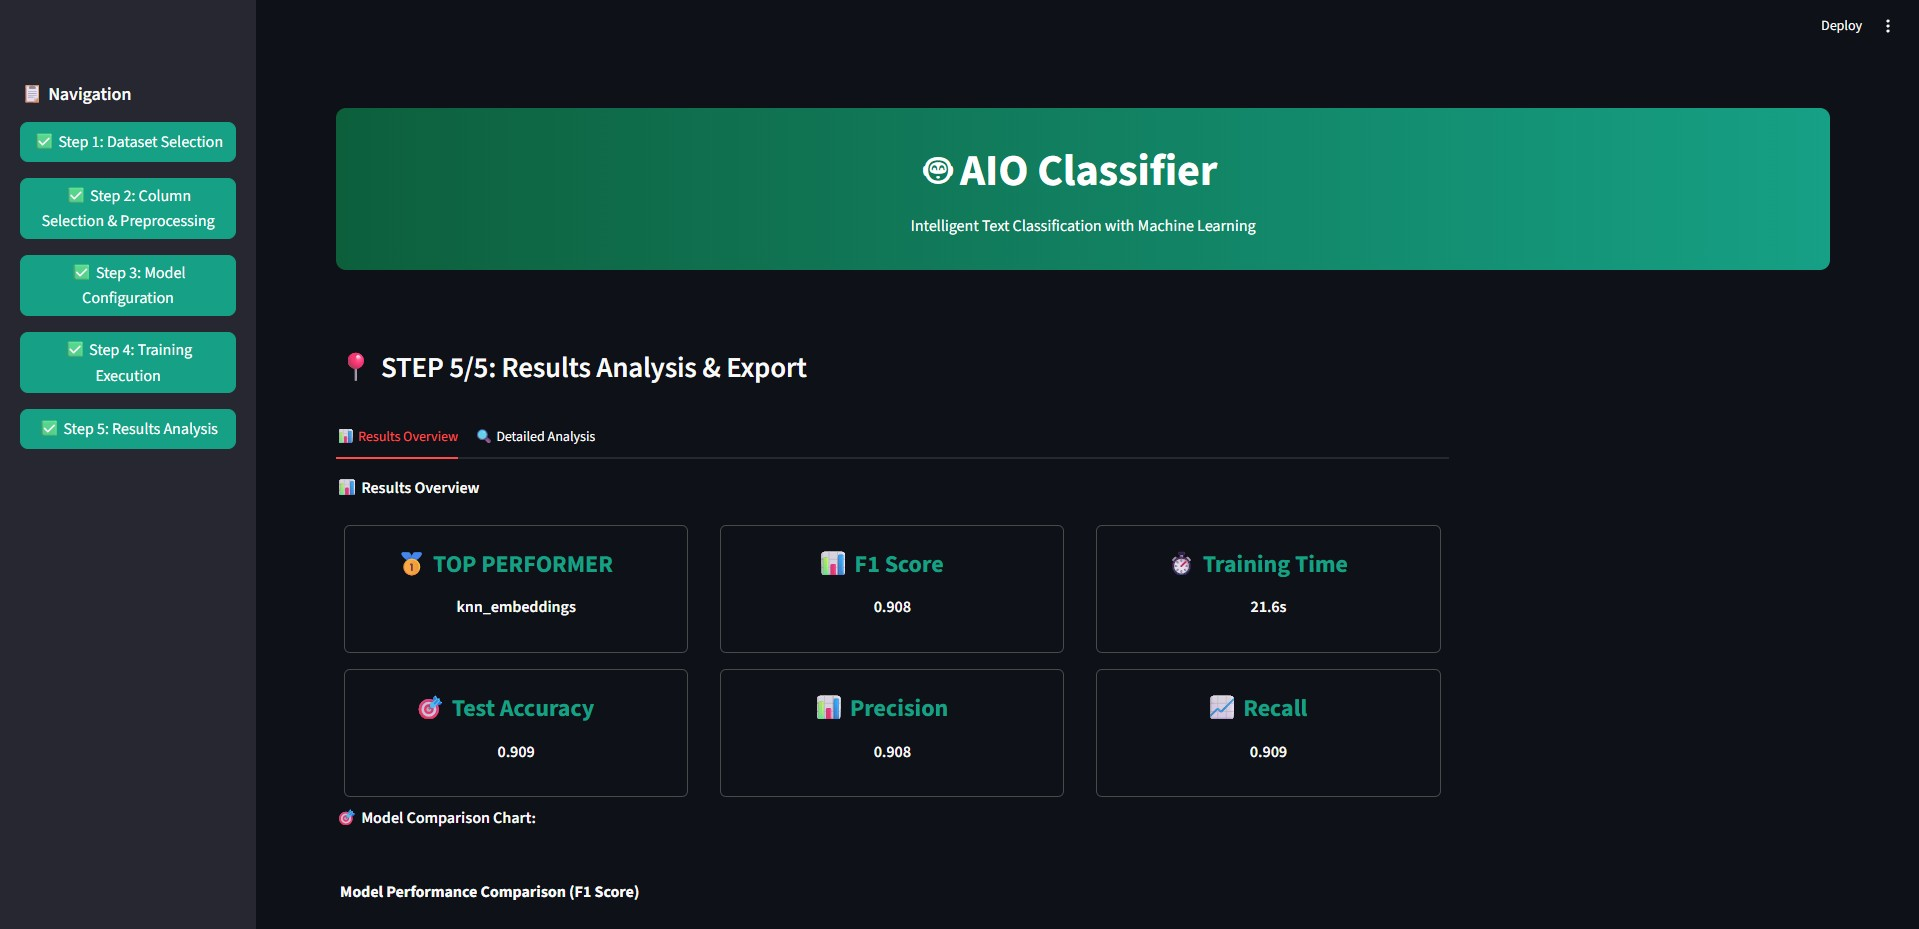
\includegraphics[width=0.9\textwidth]{image/Step 5 -1.jpg}
    \caption{Bước 5: Phân tích Kết quả và Xuất dữ liệu - Tab Tổng quan}
    \label{fig:step5-overview}
\end{figure}

\textbf{Tính năng chính:}
\begin{itemize}
    \item \textbf{Thẻ chỉ số hiệu suất:} Mô hình tốt nhất (knn\_embeddings), F1 Score (0.908), Thời gian Training (21.6s)
    \item \textbf{So sánh mô hình:} Test Accuracy (0.909), Precision (0.908), Recall (0.909)
    \item \textbf{Theo dõi tiến trình:} Tất cả 5 bước hoàn thành với dấu tích xanh
    \item \textbf{Điều hướng Tab:} Tab Tổng quan Kết quả và Phân tích Chi tiết
    \item \textbf{Chỗ dành cho trực quan hóa:} Biểu đồ so sánh mô hình và các vùng so sánh hiệu suất
\end{itemize}

\textbf{Các thành phần giao diện:}
\begin{itemize}
    \item Các thẻ chỉ số hiệu suất với thống kê chính
    \item Vùng biểu đồ so sánh mô hình (chỗ dành cho trực quan hóa)
    \item Panel điều hướng hiển thị tất cả các bước đã hoàn thành
    \item Giao diện tab để chuyển đổi giữa tổng quan và phân tích chi tiết
    \item Bố cục sạch sẽ, có tổ chức làm nổi bật mô hình hoạt động tốt nhất
\end{itemize}

\subsubsection{Bước 5: Phân tích Kết quả và Xuất dữ liệu - Phân tích Chi tiết}

\begin{figure}[H]
    \centering
    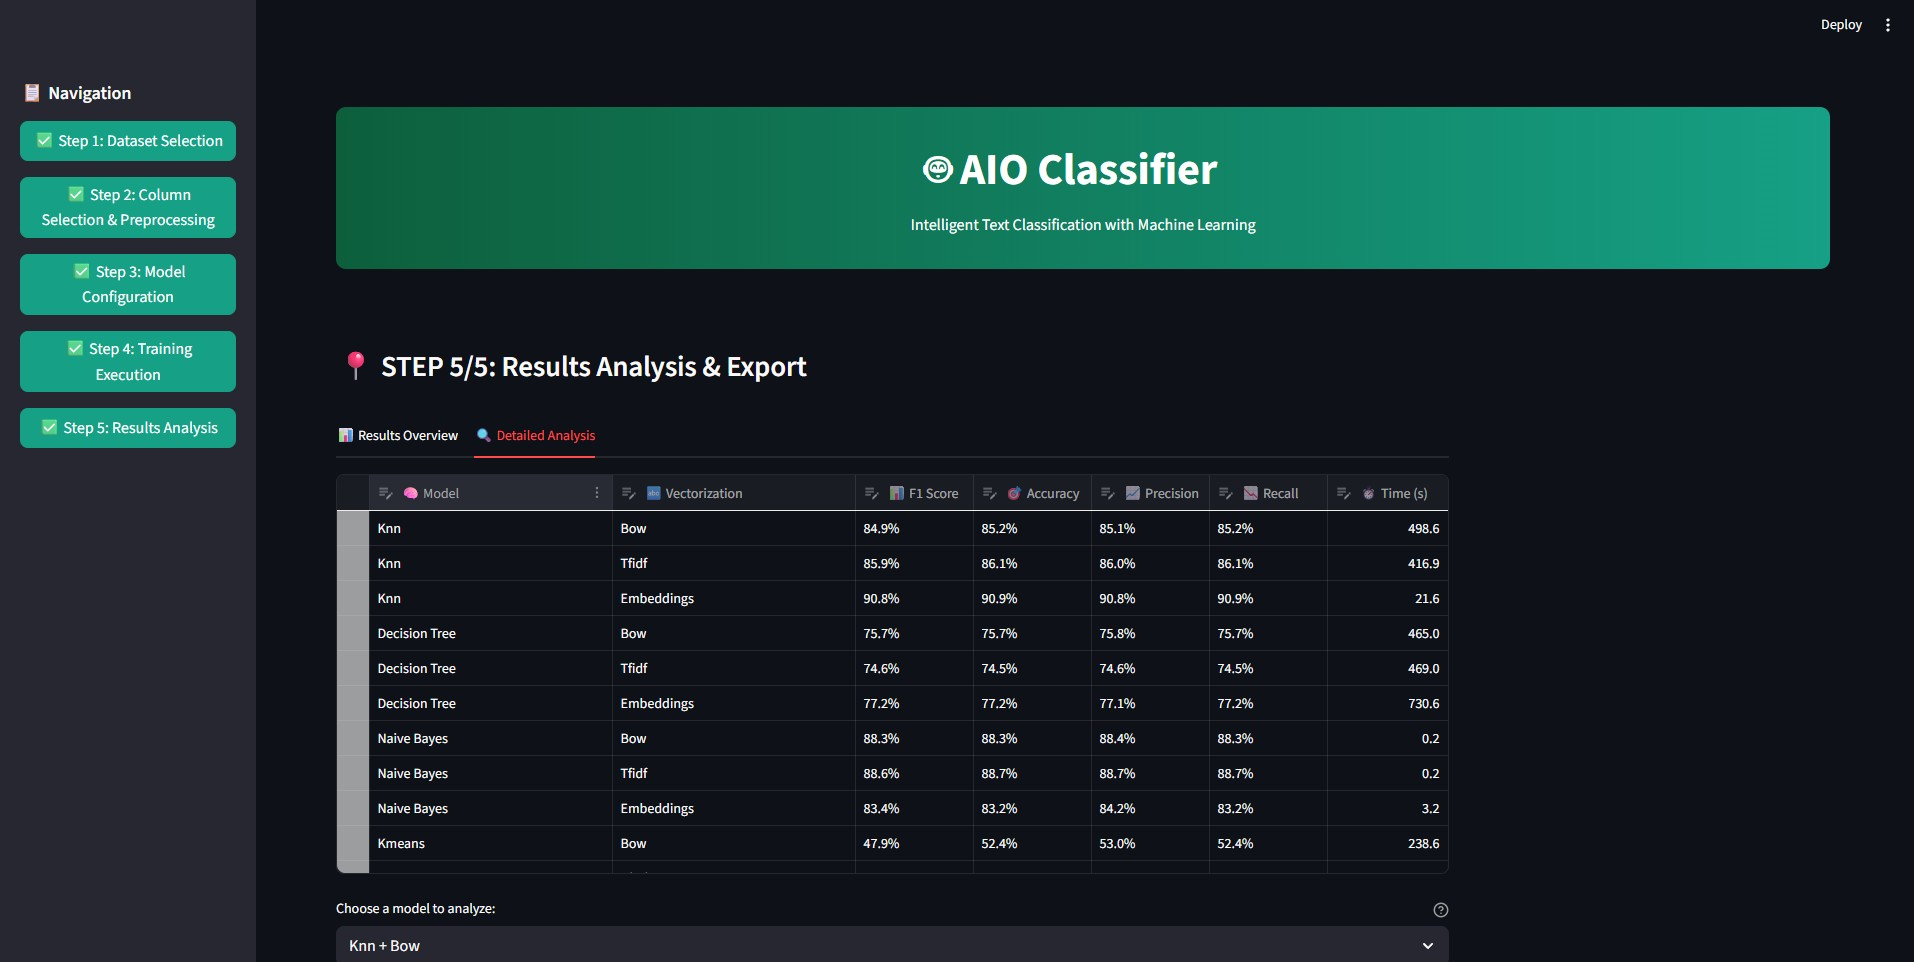
\includegraphics[width=0.9\textwidth]{image/Step 5 -2.jpg}
    \caption{Bước 5: Phân tích Kết quả và Xuất dữ liệu - Tab Phân tích Chi tiết}
    \label{fig:step5-detailed}
\end{figure}

\textbf{Tính năng chính:}
\begin{itemize}
    \item \textbf{Bảng kết quả toàn diện:} Chỉ số hiệu suất cho tất cả kết hợp mô hình-vectorization
    \item \textbf{Dropdown lựa chọn mô hình:} Chọn mô hình cụ thể để phân tích chi tiết (Knn + Bow được chọn)
    \item \textbf{So sánh hiệu suất:} Các cột F1 Score, Accuracy, Precision, Recall và Training Time
    \item \textbf{Mô hình tốt nhất được làm nổi bật:} Knn + Embeddings cho thấy hiệu suất tốt nhất (90.8\% F1 score)
    \item \textbf{Quy trình hoàn chỉnh:} Tất cả 5 bước hoàn thành với phân tích kết quả cuối cùng
\end{itemize}

\textbf{Các thành phần giao diện:}
\begin{itemize}
    \item Bảng kết quả chi tiết với 10 kết hợp mô hình khác nhau
    \item Chỉ số hiệu suất cho thấy Knn + Embeddings là mô hình tốt nhất
    \item Dropdown lựa chọn mô hình để phân tích từng mô hình riêng lẻ
    \item Giao diện tab hiển thị "Detailed Analysis" đang hoạt động
    \item Panel điều hướng xác nhận tất cả các bước đã hoàn thành
    \item So sánh thời gian training (từ 0.2s đến 730.6s)
\end{itemize}



\subsection{Responsive Design \& User Experience}

\subsubsection{Progress Tracking}

\begin{minted}{python}
def render_progress_tracker(session_manager: SessionManager):
    """Render wizard progress tracker"""
    steps = [
        "Dataset Selection",
        "Preprocessing",
        "Column Selection", 
        "Model Configuration",
        "Training Execution",
        "Results Analysis",
        "Text Classification"
    ]
    
    # Create progress bar
    progress = len(session_manager.completed_steps) / len(steps)
    st.progress(progress)
    
    # Create step indicators
    cols = st.columns(len(steps))
    
    for i, (col, step) in enumerate(zip(cols, steps)):
        with col:
            step_num = i + 1
            status = session_manager.get_step_status(step_num)
            
            if status == "completed":
                st.success(f"✅ {step_num}")
            elif status == "current":
                st.info(f"🔄 {step_num}")
            elif status == "pending":
                st.warning(f"⏳ {step_num}")
            else:
                st.error(f"🔒 {step_num}")
            
            st.caption(step)
\end{minted}

\subsection{So sánh với Notebook ban đầu}

\begin{table}[H]
\centering
\begin{tabular}{|l|c|c|}
\hline
\textbf{Aspect} & \textbf{Notebook} & \textbf{Wizard Interface} \\
\hline
User Type & Developers only & End users \\
\hline
Learning Curve & High & Low \\
\hline
Error Handling & Basic & Comprehensive \\
\hline
Progress Tracking & Manual & Automatic \\
\hline
Session Management & None & Full persistence \\
\hline
Validation & Manual & Automatic \\
\hline
Visualization & Static & Interactive \\
\hline
Export Options & Limited & Multiple formats \\
\hline
Accessibility & Code required & Point-and-click \\
\hline
\end{tabular}
\caption{So sánh Notebook vs Wizard Interface}
\end{table}

\subsection{Ưu điểm của Wizard Interface}

\begin{enumerate}
    \item \textbf{User-Friendly}: Không cần coding knowledge
    \item \textbf{Guided Workflow}: 5 bước rõ ràng, dễ follow
    \item \textbf{Real-time Feedback}: Immediate validation và error messages
    \item \textbf{Session Persistence}: Có thể save và resume work
    \item \textbf{Interactive Visualizations}: Dynamic charts và plots
    \item \textbf{Export Capabilities}: Multiple output formats
    \item \textbf{Responsive Design}: Works on different screen sizes
    \item \textbf{Error Recovery}: Graceful error handling và recovery
\end{enumerate}

\subsection{Nhược điểm và Trade-offs}

\begin{enumerate}
    \item \textbf{Complexity}: Code phức tạp hơn nhiều
    \item \textbf{Performance}: Có overhead từ UI components
    \item \textbf{Flexibility}: Ít flexible hơn direct code access
    \item \textbf{Debugging}: Khó debug UI issues
    \item \textbf{Maintenance}: Cần maintain UI code
\end{enumerate}

\subsection{Kết luận}

Wizard Interface đại diện cho một bước tiến quan trọng trong việc democratize machine learning. Nó chuyển đổi project từ một research tool thành một production-ready platform accessible cho non-technical users, đồng thời vẫn giữ được tính linh hoạt và power của underlying ML algorithms.
